% (3) 2 Different Benchmarks to Evaluate the approach as a whole and to demonstrate how the different options of the dtreeviz library impact the performance of the visualization approach:
% - French Royalty
% - Clarify
This section is meant to summarize the previous results by applying them to the non-synthetic benchmarks (\textit{The French Royalty KG} (FR-KG) and \textit{The Lung Cancer KG} (LC-KG)). Furthermore, research question \textbf{Q5} is answered based on these benchmarks. The InterpretME pipeline from section \ref{section_interpretme} is applied to the benchmarks while measuring the time spent on the different stages of the validation engine and the visualization algorithm as in the previous sections. After InterpretME extracts the dataset from the endpoint, the dataset is prepared for training of the model (e.g., removing duplicates, under-sampling, encoding categorical features, and feature selection). Table \ref{tab:samples_nodes} shows the number of samples and the number of unique seed nodes in the datasets before and after the preparation. In each run of the benchmark the decision tree, trained with the prepared dataset, is visualized; annotated once for each constraint with the constraint validation results of the constraint, and once annotated with all constraint validation results using the concept of coverage (see section \ref{section_visualizing_multiple_constraint_validation_results}). 

\begin{table}
    \centering
    \begin{tabular}{c|cccc}
        \toprule
        benchmark & \multicolumn{2}{c}{\#samples} & \multicolumn{2}{c}{\#nodes}\\
        & before prep. & after prep. & before prep. & after prep.\\
        \midrule
        \midrule
        \textit{LC-KG} & 2,102 & 428  &  1,083 & 295 \\
        \textit{FR-KG} & 2,212 & 1,988 & 2,212 & 1,988 \\
        \bottomrule
    \end{tabular}
    \caption{Number of samples and seed nodes of the extracted dataset for the non-synthetic benchmarks before preparation through the InterpretME pipeline and afterwards.}
    \label{tab:samples_nodes}
\end{table}

\paragraph{The Validation Engine} needs to be executed once for each benchmark. Figure \ref{fig:join_shacl_real_world_application} presents the execution times for the different heuristics and strategies evaluated in section \ref{section_evaluation_validation_engine} for the two non-synthetic benchmarks. The execution time spent on executing the join is lower when joining $T$ at the end. This is the expected outcome since the strategy has already shown to excel in cases the distribution of entities to classes is chosen in a way that encourages the production of constantly growing intermediate results or the number of samples is relatively low (the answer to \textbf{Q1}; see section \ref{section_evaluation_validation_engine_join}). The latter criterion applies to both benchmarks (see Figure \ref{tab:samples_nodes}) and in the case of \textit{The French Royalty KG} all target shapes of the constraints are targeting partially overlapping subsets of entities of the class \uri{dbo:Person}. Optimizing the order of the join operations does not impact positively but only adds a marginal overhead.

The heuristics to reduce the number of shapes can be applied to the SHACL shape schemas of the constraints in \textit{The Lung Cancer KG}. Each shape schema contains three shapes of which only two are required and indeed the execution time decreases when applying the heuristic. 
However, the other available heuristics cannot impact positively: In both cases, the target definitions of the target shapes of the constraints are already subsets of the set of seed nodes and simultaneous constraint validation is not applicable as none of the constraints share the SHACL shape schema. Instead, it can be seen that generating the seed query from the dataset generating query, as shown in section \ref{section_shaclapi}, adds an overhead to the SHACL validation. This is due to the execution of expensive queries generated by the SHACL engine while performing the SHACL validation. Specifying the seed query manually (e.g., using the $Q_s$ from section \ref{section_propositionalization}) leads to the results matching the answer to the research question \textbf{Q2}. 

Finally, the non-synthetic benchmarks show that optimizing the SHACL constraint validation impacts more than optimizing the join strategy. Further, it should be emphasized that the positive impact of the heuristic depends strongly on the shape schema and the KG (the answer to \textbf{Q2}; see section \ref{section_evaluation_validation_engine_shacl}).

\begin{figure}
    \centering
    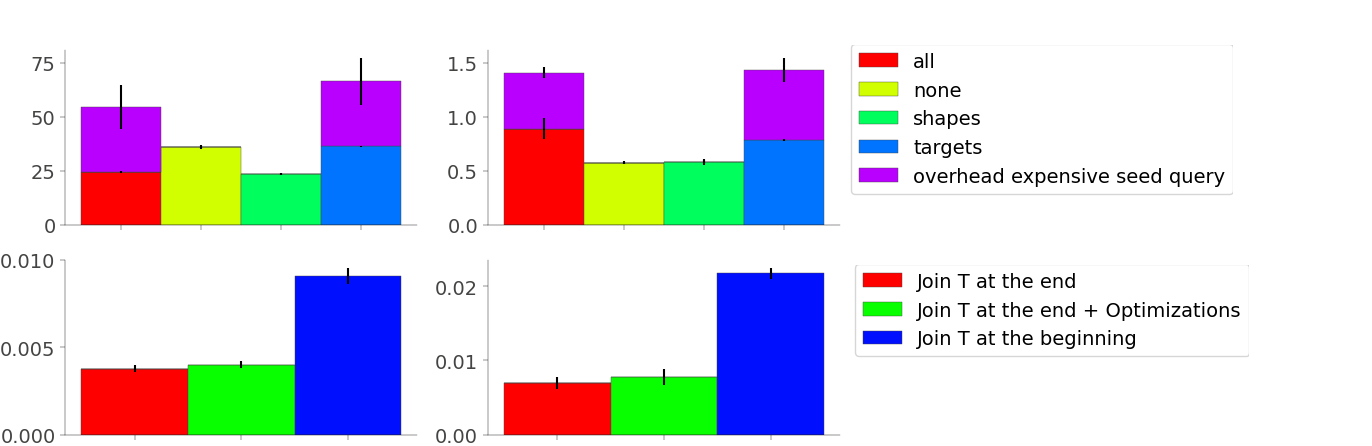
\includegraphics[width = \textwidth, trim=0 0 90 35,clip]{images/evaluation/join_shacl.png}
    \caption{Execution time [s] observed during the execution of the validation engine on performing different join strategies (at the bottom) and the SHACL validation using the different heuristics (at the top) for the non-synthetic benchmarks (FR-KG on the right and LC-KG on the left).}
    \label{fig:join_shacl_real_world_application}
\end{figure}

\paragraph{The Visualization Algorithm} is applied multiple times during the execution of the InterpretME pipeline. Figure \ref{fig:fractions_visualization_algorithm} shows the fractions of the execution time of the visualization algorithm spent for the two non-synthetic benchmarks. These portions are nearly independent of the size of the decision tree which is why the figure does not differentiate between the two benchmarks. However, the number of constraints that are visualized impacts the time needed to summarize the constraint validation results (cf. Figure \ref{fig:parallelvsserial_eval}); which can also be observed in Figure \ref{fig:fractions_visualization_algorithm}. Visualizing the decision tree with a single constraint took 3.62 seconds on average for \textit{The Lung Cancer KG} and 2.51 seconds on average for \textit{The French Royalty KG} (with standard deviations of under 0.05 seconds). This is as fast as the dtreeviz implementation or slightly faster and matches the answer to the research question \textbf{Q4} from section \ref{section_evaluation_visualization_algorithm}: The visualization algorithm excels at a larger number of samples, but scales slightly worse than dtreeviz with the size of the decision tree. 
\begin{figure}
    \centering
    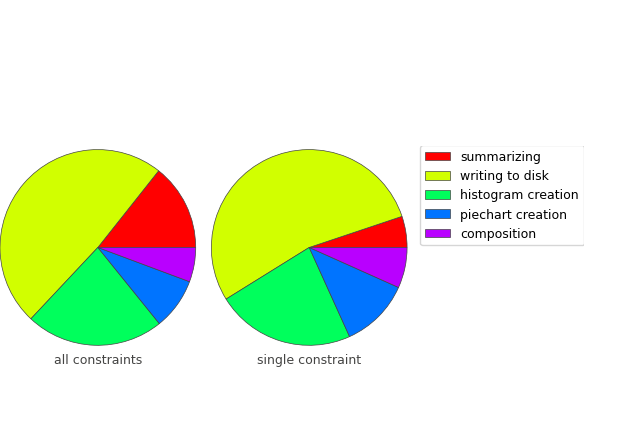
\includegraphics[width=0.7\textwidth,trim=0 50 40 100,clip]{images/evaluation/overall_viz_distribution_separate.png}
    \caption{Average portion of the execution time spent on different stages of the visualization algorithm observed for \textit{The Lung Cancer KG} and \textit{The French Royalty KG}}
    \label{fig:fractions_visualization_algorithm}
\end{figure}
When the decision tree should be annotated with the constraint validation results of multiple constraints using the coverage concept, it took 4.45 seconds on average for \textit{The Lung Cancer KG} and 3.80 seconds on average for \textit{The French Royalty KG} (with standard deviations of under 0.16 seconds). Again, it becomes obvious that the time needed to annotate the decision tree with the constraint validation results of multiple constraints grows slower than linearly with the number of constraints. 

Generating the decision tree node plot visualizations in parallel raises the execution time of the visualization algorithm when annotating the decision tree with the constraint validation results of a single constraint to 4.75 seconds on average for \textit{The Lung Cancer KG} and 4.15 seconds on average for \textit{The French Royalty KG} (with standard deviations of about 0.5 seconds). The decision tree has to be of a specific size, which grows linear with the number of samples in the dataset, to benefit from the multiprocessing implemented (the answer to \textbf{Q3}; see section \ref{section_evaluation_visualization_algorithm}).

\paragraph{Summary.} Finally, research question \textbf{Q5} asking about the overall overhead added by the validation engine and the visualization algorithm compared to the normal model training and other kinds of interpretability methods (e.g., dtreeviz and LIME) can be answered. As a reference, measurements of the execution times of the InterpretME pipeline are used; they are listed in table \ref{fig:benchmark_reference_times}. Here the overall execution time of the approach is made up of the dataset extraction, the model training, the constraint evaluation per sample in the dataset, and the visualization of the annotated decision tree. It is assumed that all constraints are used to annotate a single decision tree using the coverage concept. In the average worst-case scenario, the approach took up to 73.33 seconds (using the generated seed query; only applying the target reduction; joining $T$ at the beginning) in the case of \textit{The Lung Cancer KG} and up to 6.65 seconds in the case of \textit{The French Royalty KG} (with standard deviations of 10.86 and 1.76 seconds resp.). However, in the average best-case scenario, the approach took 30.39 and 5.8 seconds resp. (using the manually specified seed query; only pruning the shape network; joining $T$ at the end; with standard deviations of 1.18 and 0.28 seconds resp.). Regarding \textbf{Q5} that makes the execution time of using the approach up to 44 times resp. 6 times slower with respect to the model training but still up to 62 resp. 73 times faster than using LIME. Due to the large differences in execution time depending on the benchmark, no clear answer can be given. However, due to the complexity of the approach (see section \ref{section_validation_engine_complexity}) expensive scenarios will lead to a large overhead of the approach.

\begin{table}
    \centering
    \begin{tabular}{l|cccccccc}
        \toprule
        benchmark & \multicolumn{2}{c}{dataset extraction} & \multicolumn{2}{c}{model training} & \multicolumn{2}{c}{dtreeviz} & \multicolumn{2}{c}{LIME} \\
        & avg. & std. & avg. & std. & avg. & std. & avg. & std. \\
        \midrule
        \midrule
        \textit{LC-KG} & 0.77 & 0.45 & 1.68 & 0.07 & 4.05 & 0.70 & 1894.67 & 19.14 \\
        \textit{FR-KG} & 0.20 & 0.06 & 1.19 & 0.04 & 2.51 & 0.09 & 424.12 & 3.02\\
        \bottomrule
    \end{tabular}
    \caption{Reference execution times [s] measured for \textit{The French Royalty KG} (FR-KG) and \textit{The Lung Cancer KG} (LC-KG). dataset extraction -- time spent executing the dataset generating query; model training -- time spent on finding an appropriate model for the predictive task of the benchmark (includes preprocessing, sampling, feature selection, hyper parameter grid search and decision tree training); dtreeviz -- time spent to visualize the trained decision tree with dtreeviz; LIME -- time spent on calculating LIME interpretability results for a quarter of the samples in the dataset}
    \label{fig:benchmark_reference_times}
\end{table}

%0.77s + 1.68 + 66.42s + 0.01s + 4.45s = 73.33s
%0.2s + 1.19s + 1.43s + 0.02s + 3.8s = 6.65s

%0.77s + 1.68 + 23.49s + 0.004s + 4.45s = 30.39s
%0.2s + 1.19s + 0.58s + 0.007s + 3.8s = 5.8s